\documentclass{article}

\usepackage{graphicx}
\usepackage{subcaption}
\usepackage{amsmath}
\usepackage{todonotes}
\let\Cross\relax
\usepackage{cool}

%%%%%%%%%%%%%%%%%%%%%%%%%%%%%%%%%%%%%%%%%%%%%%%%%%%%%%%%%%%%%
%% LaTeX math macros
%%%%%%%%%%%%%%%%%%%%%%%%%%%%%%%%%%%%%%%%%%%%%%%%%%%%%%%%%%%%%

\newcommand{\mySetNotation}[1]{{\mathbb{#1}}}
\newcommand{\RRSet}{{\mySetNotation{R}}}
\newcommand{\EESet}{{\mySetNotation{E}}}
\newcommand{\NNSet}{{\mySetNotation{N}}}
\newcommand{\QQSet}{{\mySetNotation{Q}}}
\newcommand{\ZZSet}{{\mySetNotation{Z}}}
\newcommand{\RRR}{{\mySetNotation{R}}}


\newcommand{\myBoldNotation}[1]{{\mathbf #1}}
%\newcommand{\myBoldNotation}[1]{{\mathbold{#1}}} %for euler math
\newcommand{\va}   {{\myBoldNotation{a}}}
\newcommand{\vb}   {{\myBoldNotation{b}}}
\newcommand{\vc}   {{\myBoldNotation{c}}}
\newcommand{\vd}   {{\myBoldNotation{d}}}
\newcommand{\ve}   {{\myBoldNotation{e}}}
\newcommand{\vf}   {{\myBoldNotation{f}}}
\newcommand{\vg}   {{\myBoldNotation{g}}}
\newcommand{\vh}   {{\myBoldNotation{h}}}
\newcommand{\vi}   {{\myBoldNotation{i}}}
\newcommand{\vj}   {{\myBoldNotation{j}}}
\newcommand{\vk}   {{\myBoldNotation{k}}}
\newcommand{\vl}   {{\myBoldNotation{l}}}
\newcommand{\vm}   {{\myBoldNotation{m}}}
\newcommand{\vn}   {{\myBoldNotation{n}}}
\newcommand{\nn}   {{\myBoldNotation{n}}}
\newcommand{\vo}   {{\myBoldNotation{o}}}
\newcommand{\vp}   {{\myBoldNotation{p}}}
\newcommand{\pp}   {{\myBoldNotation{p}}}
\newcommand{\vq}   {{\myBoldNotation{q}}}
\newcommand{\vr}   {{\myBoldNotation{r}}}
\newcommand{\vs}   {{\myBoldNotation{s}}}
\newcommand{\vt}   {{\myBoldNotation{t}}}
\newcommand{\vu}   {{\myBoldNotation{u}}}
\newcommand{\vv}   {{\myBoldNotation{v}}}
\newcommand{\vw}   {{\myBoldNotation{w}}}
\newcommand{\vx}   {{\myBoldNotation{x}}}
\newcommand{\vy}   {{\myBoldNotation{y}}}
\newcommand{\vz}   {{\myBoldNotation{z}}}
\newcommand{\vNull}{{\myBoldNotation{0}}}
\newcommand{\vOne} {{\myBoldNotation{1}}}

\newcommand{\mA}   {{\myBoldNotation{A}}}
\newcommand{\mB}   {{\myBoldNotation{B}}}
\newcommand{\mC}   {{\myBoldNotation{C}}}
\newcommand{\mD}   {{\myBoldNotation{D}}}
\newcommand{\mE}   {{\myBoldNotation{E}}}
\newcommand{\mF}   {{\myBoldNotation{F}}}
\newcommand{\mG}   {{\myBoldNotation{G}}}
\newcommand{\mH}   {{\myBoldNotation{H}}}
\newcommand{\mI}   {{\myBoldNotation{I}}}
\newcommand{\mJ}   {{\myBoldNotation{J}}}
\newcommand{\mK}   {{\myBoldNotation{K}}}
\newcommand{\mL}   {{\myBoldNotation{L}}}
\newcommand{\mM}   {{\myBoldNotation{M}}}
\newcommand{\mN}   {{\myBoldNotation{N}}}
\newcommand{\mO}   {{\myBoldNotation{O}}}
\newcommand{\mP}   {{\myBoldNotation{P}}}
\newcommand{\mQ}   {{\myBoldNotation{Q}}}
\newcommand{\mR}   {{\myBoldNotation{R}}}
\newcommand{\mS}   {{\myBoldNotation{S}}}
\newcommand{\mT}   {{\myBoldNotation{T}}}
\newcommand{\mU}   {{\myBoldNotation{U}}}
\newcommand{\mV}   {{\myBoldNotation{V}}}
\newcommand{\mW}   {{\myBoldNotation{W}}}
\newcommand{\mX}   {{\myBoldNotation{X}}}
\newcommand{\mY}   {{\myBoldNotation{Y}}}
\newcommand{\mZ}   {{\myBoldNotation{Z}}}
\newcommand{\mNull}{{\myBoldNotation{0}}}
\newcommand{\mOmega}   {{\myBoldNotation{\Omega}}}

\newcommand{\myBoldGreekNotationLower}[1]{{\bm{#1}}}
\newcommand{\myBoldGreekNotationUpper}[1]{{\bm{#1}}}
\newcommand{\balpha}  {{\myBoldGreekNotationLower{\alpha}  }}
\newcommand{\bbeta}   {{\myBoldGreekNotationLower{\beta}   }}
\newcommand{\bgamma}  {{\myBoldGreekNotationLower{\gamma}  }}
\newcommand{\bdelta}  {{\myBoldGreekNotationLower{\delta}  }}
\newcommand{\bepsilon}{{\myBoldGreekNotationLower{\epsilon}}}
\newcommand{\bzeta}   {{\myBoldGreekNotationLower{\zeta}   }}
\newcommand{\btheta}  {{\myBoldGreekNotationLower{\theta}  }}
\newcommand{\biota}   {{\myBoldGreekNotationLower{\iota}   }}
\newcommand{\bkappa}  {{\myBoldGreekNotationLower{\kappa}  }}
\newcommand{\blambda} {{\myBoldGreekNotationLower{\lambda} }}
\newcommand{\bmu}     {{\myBoldGreekNotationLower{\mu}     }}
\newcommand{\bnu}     {{\myBoldGreekNotationLower{\nu}     }}
\newcommand{\bxi}     {{\myBoldGreekNotationLower{\xi}     }}
\newcommand{\bomicron}{{\myBoldGreekNotationLower{\omicron}}}
\newcommand{\bpi}     {{\myBoldGreekNotationLower{\pi}     }}
\newcommand{\brho}    {{\myBoldGreekNotationLower{\rho}    }}
\newcommand{\bsigma}  {{\myBoldGreekNotationLower{\sigma}  }}
\newcommand{\btau}    {{\myBoldGreekNotationLower{\tau}    }}
\newcommand{\bupsilon}{{\myBoldGreekNotationLower{\upsilon}}}
\newcommand{\bphi}    {{\myBoldGreekNotationLower{\phi}    }}
\newcommand{\bchi}    {{\myBoldGreekNotationLower{\chi}    }}
\newcommand{\bpsi}    {{\myBoldGreekNotationLower{\psi}    }}
\newcommand{\bomega}  {{\myBoldGreekNotationLower{\omega}  }}

\newcommand{\mLambda} {\Lambda}
\newcommand{\mSigma} {\Sigma}

\newcommand{\bGamma}  {{\myBoldGreekNotationUpper{\Gamma}  }}
\newcommand{\bDelta}  {{\myBoldGreekNotationUpper{\Delta}  }}
\newcommand{\bTheta}  {{\myBoldGreekNotationUpper{\Theta}  }}
\newcommand{\bLambda} {{\myBoldGreekNotationUpper{\Lambda} }}
\newcommand{\bXi}     {{\myBoldGreekNotationUpper{\Xi}     }}
\newcommand{\bPi}     {{\myBoldGreekNotationUpper{\Pi}     }}
\newcommand{\bSigma}  {{\myBoldGreekNotationUpper{\Sigma}  }}
\newcommand{\bUpsilon}{{\myBoldGreekNotationUpper{\Upsilon}}}
\newcommand{\bPhi}    {{\myBoldGreekNotationUpper{\Phi}    }}
\newcommand{\bPsi}    {{\myBoldGreekNotationUpper{\Psi}    }}
\newcommand{\bOmega}  {{\myBoldGreekNotationUpper{\Omega}  }}

\newcommand{\inn}[2][0cm]{\mathopen{}\left|{#2}\parbox[h][#1]{0cm}{}\right|}
\newcommand{\invn}[2][0cm]{\mathopen{}\left|\left|{#2}\parbox[h][#1]{0cm}{}\right|\right|}

%\newcommand{\Sa}{{\mathbf {Sa}}}
%\newcommand{\Topo}{{\mathbf {Topo}}}
%\newcommand{\Sep}{{\mathbf {Sep}}}
%\newcommand{\Str}{{\mathbf {Str}}}
%\newcommand{\Reg}{{\mathbf {Reg}}}

%\newcommand{\PPhi}{{\pmb \Phi}}
%\newcommand{\PPi}{{\pmb \Pi}}
%\newcommand{\PPhi}{{\bm \Phi}}
%\newcommand{\PPi}{{\bm \Pi}}
\newcommand{\PPhi}{{\Phi}}
\newcommand{\PPi}{{\Pi}}
\newcommand{\ppi}{{\pi}}
\newcommand{\ggam}{{\gamma}}

\newcommand{\cA}{{\mathcal A}}
\newcommand{\cB}{{\mathcal B}}
\newcommand{\cC}{{\mathcal C}}
\newcommand{\cD}{{\mathcal D}}
\newcommand{\cE}{{\mathcal E}}
\newcommand{\cF}{{\mathcal F}}
\newcommand{\cG}{{\mathcal G}}
\newcommand{\cH}{{\mathcal H}}
\newcommand{\cI}{{\mathcal I}}
\newcommand{\cJ}{{\mathcal J}}
\newcommand{\cK}{{\mathcal K}}
\newcommand{\cL}{{\mathcal L}}
\newcommand{\cM}{{\mathcal M}}
\newcommand{\cN}{{\mathcal N}}
\newcommand{\cO}{{\mathcal O}}
\newcommand{\cP}{{\mathcal P}}
\newcommand{\cQ}{{\mathcal Q}}
\newcommand{\cR}{{\mathcal R}}
\newcommand{\cS}{{\mathcal S}}
\newcommand{\cT}{{\mathcal T}}
\newcommand{\cU}{{\mathcal U}}
\newcommand{\cV}{{\mathcal V}}
\newcommand{\cW}{{\mathcal W}}
\newcommand{\cX}{{\mathcal X}}
\newcommand{\cY}{{\mathcal Y}}
\newcommand{\cZ}{{\mathcal Z}}

\newcommand{\ca}{{\mathcal a}}
\newcommand{\cb}{{\mathcal b}}
\newcommand{\cc}{{\mathcal c}}
\newcommand{\cd}{{\mathcal d}}
\newcommand{\ce}{{\mathcal e}}
%\newcommand{\cf}{{\mathcal f}}
\newcommand{\cg}{{\mathcal g}}
\newcommand{\ch}{{\mathcal h}}
\newcommand{\ci}{{\mathcal i}}
\newcommand{\cj}{{\mathcal j}}
%\newcommand{\ck}{{\mathcal k}}
\newcommand{\cl}{{\mathcal l}}
\newcommand{\cm}{{\mathcal m}}
\newcommand{\cn}{{\mathcal n}}
\newcommand{\co}{{\mathcal o}}
\newcommand{\cp}{{\mathcal p}}
\newcommand{\cq}{{\mathcal q}}
%\newcommand{\cr}{{\mathcal r}}
\newcommand{\cs}{{\mathcal s}}
\newcommand{\ct}{{\mathcal t}}
\newcommand{\cu}{{\mathcal u}}
\newcommand{\cv}{{\mathcal v}}
\newcommand{\cw}{{\mathcal w}}
\newcommand{\cx}{{\mathcal x}}
\newcommand{\cy}{{\mathcal y}}
\newcommand{\cz}{{\mathcal z}}

%cool package Styles
\Style{IdentityMatrixSymb=\mI,%
       DSymb={\mathrm d},%
       IntegrateDifferentialDSymb={\mathrm d},%
       TrParen=p,%
       DetParen=p}
\Style{DDisplayFunc=outset}
\renewcommand{\Transpose}[1]{ {#1}^\Transp }
\newcommand{\TransposeInv}[1]{ {#1}^{-\Transp} }
\newcommand{\T}[1]{\Transpose{#1}}
\newcommand{\TInv}[1]{\TransposeInv{#1}}
\newcommand{\Inv}[1]{ {#1}^{-1} }
\newcommand{\Transp}{{{\mathrm T}}}
\newcommand{\Norm}[1]{\left\lVert#1\right\rVert}

\newcommand{\Rank}[1]    {\operatorname{rank}\inp{#1}}
\newcommand{\Vol}[1]     {\operatorname{vol}\inp{#1}}
\renewcommand{\Vec}[1]   {\operatorname{vec}\inp{#1}}
\renewcommand{\Div}[1]   {\T{\nabla} \, #1}
\newcommand{\Diag}[1]    {\operatorname{diag}\inp{#1}}
\newcommand{\Dim}[1]     {\operatorname{dim}\inp{#1}}
\newcommand{\Diagof}[1]  {\operatorname{diag}^{-1}\inp{#1}}
\newcommand*{\diff}{\mathop{}\!\mathrm{d}} %e.g. $F(x) = \int\!f(x)\diff x$
\newcommand{\Argmin}[1]{\underset{#1}{\operatorname{argmin}} \;}
\newcommand{\Maxof}[1]{\underset{#1}{\operatorname{max}} \;}
\newcommand{\Minof}[1]{\underset{#1}{\operatorname{min}} \;}

\providecommand{\e}[1]{\ensuremath{\cdot 10^{#1}}}

%workaround for mathbold in cool, cf. http://tex.stackexchange.com/questions/97910
%\let\oldmb\mathbold
%\protected\def\mathbold{\oldmb}

\newcommand{\CB} [1]{{\color{#1}     $\bullet$}}
\newcommand{\CBB}[2]{{\color[#1]{#2} $\bullet$}}

\newcommand{\ie}{i.e.}
\newcommand{\Ie}{I.e.}
\newcommand{\eg}{e.g.}
\newcommand{\Eg}{E.g.}
\newcommand{\cf}{cf.\ }
\newcommand{\Cf}{Cf.\ }
\newcommand{\etc}{etc.\ }
\newcommand{\wrt}{w.r.t.\ }
\newcommand{\Wrt}{W.r.t.\ }
\newcommand{\Wlog}{W.l.o.g.\ }
\newcommand{\resp}{resp.\ }
\newcommand{\etal}{et al.\ }

% \newtheorem{theorem}{Theorem}
% \newtheorem{definition}{Definition}
% \newtheorem{expectation}{Expectation}
% \newtheorem{problem}{Problem}
% %\newtheorem{algorithm}{Algorithm}


% http://tex.stackexchange.com/questions/145716/underbrace-in-a-matrix
\newcommand{\underbracedmatrix}[2]{%
  \left(\;
  \smash[b]{\underbrace{
    \begin{matrix}#1\end{matrix}
  }_{#2}}
  \;\right)
  \vphantom{\underbrace{\begin{matrix}#1\end{matrix}}_{#2}}
}

\title{Bone Cement Volumetry in sagittal and axial MRT-Images of the Spine}

\author{Friederici Anke\\ Jordan Grigori}

\begin{document}
  
  \begin{titlepage}
    \centering
    
  \end{titlepage}
  
  \maketitle
  \thispagestyle{empty}
%  \pagebreak
  
  \section{Introduction}
  \setcounter{page}{1}
  {
    We were introduced to the problem of semiautomatic bone cement volumetry 
    on MR-images of a spline.
    Our application is required 
    to detect such regions of the spine reliably to allow for volumetric measurements.\\
    \\The data that is given presents the challenge, MR-images, which do not have
    the strong contrast of CT-images nor are as noise free as CT-images, when it
    comes to bone tissue. Thus more image processing becomes necessary to possibly 
    achieve equally as good result as working with CT data.
    At its core this is a non trivial segmentation task, which requires a thought 
    through choice of image processing and segmentation algorithms.\\
    \\Our approach was to split the solution to the problem in two steps:
    \begin{enumerate}
      \item Single out one vertebra of choice, by user input (e.g. a single mouse click).
      \item Segment the chosen vertebra to its extent over the MR-images and measure the hollow regions volume, as precise as possible.
    \end{enumerate}
    We decided to keep it as simple as possible, by implementing the task at hand 
    entirely on Matlab. 
    As we are faced with possibly very uncommonly-shaped regions, we chose \textit{Normalized Graph Cuts} \cite{[ShiMalik00]} as our segmentation algorithm.
    It is heavily based on matrix operations and does not enforce any 'roundness' of the result.
    \\Matlab also has its own implementation of an active contour
    operation \cite{[ChanVese01]}, which could be used to segment the vertebra needed to a satisfying degree for the actual task of bone cement volumetry.\\	
    \\In the following chapters we will first describe how we implemented the vertebra segmentation.
    Afterwards, we will move on to describing our chosen filling compound segmentation inside the vertebra.
    At last in the remaining two chapters we will present our results and evaluate them, to see how well our application fare against the ground truth solution.
    on MR-images of a spline.
  }
%  \pagebreak
  \section{Vertebra Segmentation}
  {
    The implementation of the vertebra segmentation makes solely use of features and algorithms
    of Matlab. At first we let the user select a vertebra interactively. For that purpose a basic 
    dicom slice viewer is available, to first let the user decide, which slide he sees fitting to select the ROI. In the next step via, currently two clicks, the user chooses at last the ROI, marking the left upper and the right lower region of the desired vertebra.\\
    \\In the next stage the actual vertebra segmentation takes place, using the \textit{Chan-Vese Segmentation} \cite{[ChanVese01]}, which is an active contour algorithm without edges. It is based on a simplified \textit{Mumford-Shah Model} \cite{[MumfordShah89]}, it requires the approximated function to be piecewise constant instead of smooth and further more results in a binary approximation. The segmentation boundary is represented implicitly by a level set function. The contour of the segmentation is iteratively found by a gradient descent. \\
    \\ The Matlab implementation of this algorithm provides two parameters, the first one, 'SmoothFactor', which allows us to control the shape of the resulting segmentation and the second being the count of iterations for the evolution of the contour.
    Low values of 'SmoothFactor', below 0, allow for finer details to come through, whereas higher values might smooth over details. For our purpose 3.0 was the value of choice for the 'SmoothFactor' parameter and a count of 200 for the iterations, to achieve satisfying vertebra segmentation results.\\
    \\For improved vertebra segmentation the T1 plus contrast-agent and T2 MR-sequences are used, by obtaining a segmentation mask with the \textit{Chan-Vese Segmentation} \cite{[ChanVese01]} on each corresponding user chosen MR-slice. Multiplying both obtained mask results in a satisfactory segmentation of the vertebra.  
    Initially in order to obtain the remaining masks on the MR-sequence, containing the chosen vertebra and make volumetric measurement of bone cement treatment region possible we applied the \textit{Chan-Vese Segmentation} \cite{[ChanVese01]} on each MR-slice. \newline 
    We did it in two ways, away from the initially chosen slice. In this process the input mask for the current slice to apply the segmentation algorithm on is always the first resulting segmentation. To further refine the result a function was implemented, by which we attempt is to discard segmentation computation based on three criteria:
    \begin{enumerate}
    	\item Number of segment components (must be one).
    	\item Comparison of the minimal bounding box extent of the new segmentation to the first computed result.
    	\item Comparison of the position of the 'center points' (sum of all segment coordinates and divide by their count) of the new segmentation to the first computed result. 
    \end{enumerate}
	If one criteria is above a certain threshold then the segmentation from the current slice index will not be applied. This function does not work completely on all vertebra, but in case of uncertainty the segmentation algorithm is applied on all MR-images to ensure, that the whole vertebra is contained. Suitable thresholds were acquired through testing.\\
    \begin{figure}[h]
      \centering
      \begin{subfigure}[t]{0.45\linewidth}
        \centering
        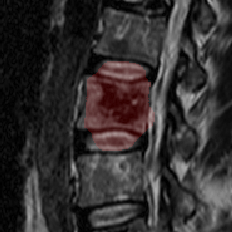
\includegraphics[scale=1.4]{VertebraSegmentationExample_1.png}
        
      \end{subfigure}
      \hfill
      \begin{subfigure}[t]{0.45\linewidth}
        \centering
        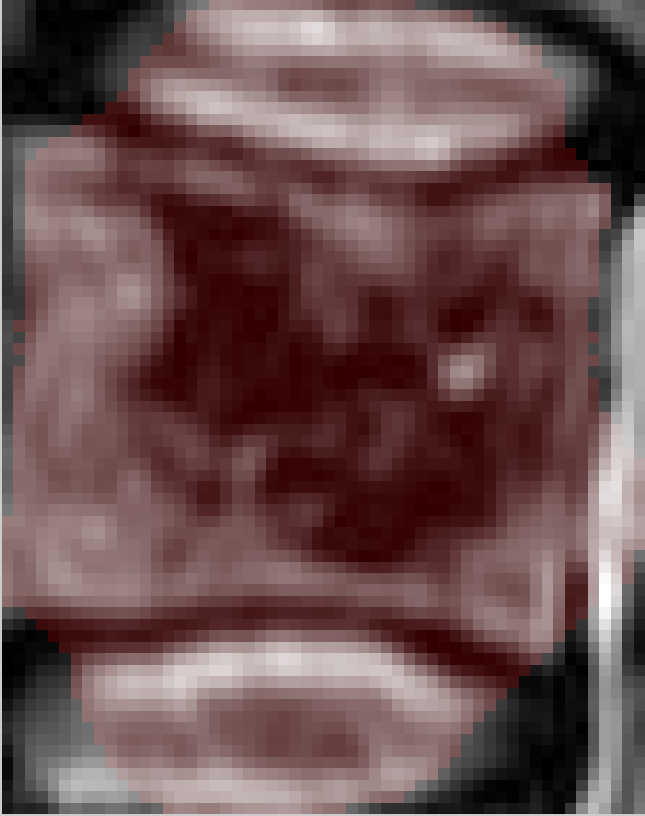
\includegraphics[scale=0.4]{VertebraSegmentationExample_2.png}
      \end{subfigure}
      \caption{Vertebra Segmentation Example\\
        \textit{The segmented area containing the cement region is highlighted in red. For further processing, the data is shrunk to the minimal box enclosing the mask.}}
    \end{figure} 
  }	
  
%  \pagebreak
  \section{Filling Compound Segmentation}
  
  Within this rough segmentation of the vertebra body, we now search for the bone cement structures.
  In this reduced dataset, we are faced with a relatively low resolution (approximately $50 \times 40$ pixels $\times 15$ slices), high inhomogeneities due to the porous structure of bones and irregular structures to be segmented.
  The holes filled with bone cement show as low-valued areas.
  Due to partial volume effects, the edges are not sharp. 
  
  Taking all this together, we decided to try \textit{Normalized Graph Cuts} as described by Shi and Malik~\cite{[ShiMalik00]} as segmentation algorithm.
  Basically, the image is represented as a non-directed, weighted graph, with pixels and inter-pixel similarities corresponding to nodes and weights respectively.
  Representing the graph to a Laplacian matrix, we are able to compute the \textit{real-valued minimal normalized cut} by solving an eigenvector problem on a similarity graph.
  
  \subsection*{Normalized Graph Cut}
    For computation, we set up
    
  \begin{equation*}
  \begin{alignedat}{2}
  \mW_{ij} &= w_{ij} \\
  \mD_{ii} &= \sum_j w_{ij} .
  \end{alignedat}
  \end{equation*}
  $\mW$ is the connectivity matrix, symmetric semi-positive definite by construction.
  $\mD$ is a diagonal matrix storing the total connectivity per point.
  The weights $w_{ij}$ are to be filled with a measure of similarity.
  This is basically the only tunable parameter of the method.
  
  The \textit{normalized cut} of two segments A and B is defined as the connectivity between A and B, normalized by the total connectivity of each segment, or
  \begin{equation}\label{eq:mincut}
    \frac{\sum_{a \in A,b \ in B} w_{ab}}
    {\sum_{a \in A, v \in A \cup B} w_{av}} + 
      \frac{\sum_{a \in A,b \ in B} w_{ab}}
      {\sum_{b \in B, v \in A \cup B} w_{bv}}
  \end{equation}
 
  
  Based on $\mW$ and $\mD$, the \textit{real-valued minimal normalized cut} of the graph can be found by solving
  \begin{equation}
    (\mD-\mW) y = \lambda \mD y
  \end{equation}
  for minimal $y$, \ie~by solving a Laplacian matrix for the eigenvector with the smallest corresponding eigenvalue (omitting the first eigenvector-eigenvalue pair, $\{\textbf{1}, 0\}$).
  This $y_{min}$ will have the property of minimizing the total cut, where $1$ and $-1$ indicate the two segments.
  %each value represents the affiliation to the $1$ or $-1$ segment.
  To extract the optimal \textit{binary} segmentation from this field, Shi and Malik suggest to simply try out several threshold values on $y_{min}$ and applying the one minimizing equation \ref{eq:mincut}.
  
  \subsection*{Connectivity Matrix Setup}
  As mentioned above, the only exchangeable parameter in the method is $w_{ij}$, the similarity between pixels.
  We followed the example given by Shi and Malik. Within a set neighborhood, similarity is defined as difference in value divided by distance:
  \begin{equation}
    w_{ij} = \frac{1}{dist(i,j)}~
    e^{\frac{-\Norm{X_i - X_j}^2}{\sigma^2_X}}
  \end{equation}
  where $X_i$ is the image value at position $i$ and $\sigma^2_X$ is the overall variance of all $X_i$.
  We chose a neighborhood of up to $8$ pixels in each direction and up to $\lceil\frac{8}{6}\rceil=2$ slices to account for the difference in element distance.
  More neighbors add more non-zero values to $\mW$, but do not increase its size. So, as solving becomes slower, it is also stabilized.
  
  \subsection{Iterative Segmentation}
  As the matrices involved are symmetric, all eigenvalues are orthogonal.
  This means that while the second smallest eigenvalue can be used to cut the area in half, the next eigenvectors cut the resulting segments optimally again.
  Shi and Malik mention the instability of this approach.
  Cuts become more expensive and less accurate the higher the eigenvalue gets.
  
  Taking this into account, we implemented 4 different possibilities for iterative segmentation:
  \begin{enumerate}
    \item
    Using the $n$ smallest eigenvalues, the area is segmented into approximately $2^n$ segments.
    This variant results in several small segments and performs worse the higher $n$ becomes.
    For $n = 1$, only one cut is performed, which is the basis for the other versions.
    For a simple example, see figure~\ref{fig:eigen}.
    \item
    Instead of solving the system once for $n$ eigenvalues, we can also recursively subdivide the segments.
    This basically means computing eigenvalues of a submatrix and evaluating equation \ref{eq:mincut} in a smaller area.
    However, the segments will not always be of the same size, result in segments of highly varying size.
    \item
    To circumvent this problem, one can always split the segment with the highest area, until a certain segment size or iteration count is reached.
    This however tends to cut uniform areas more often than necessary, while interesting areas tend to have a smaller area.
    \item
    In order to integrate this property, we decided to choose the segment with highest variance as splitting candidate.
    To ignore high variances in higher image values, we clamp them to approximately double the highest cement value.
    For a simple example, see figure~\ref{fig:minvar}.
  \end{enumerate}
  
  As we can reuse the system matrix in all cases, they are not considerably different in computational complexion.
  The first version is the most simple and slightly faster (as we do not need to partition the system and only once split non-connected regions with the same segment ID) and was thus used when the matrix became more dense (in 3D or in a larger neighborhood).
  
  \begin{figure}[h]
    \centering
    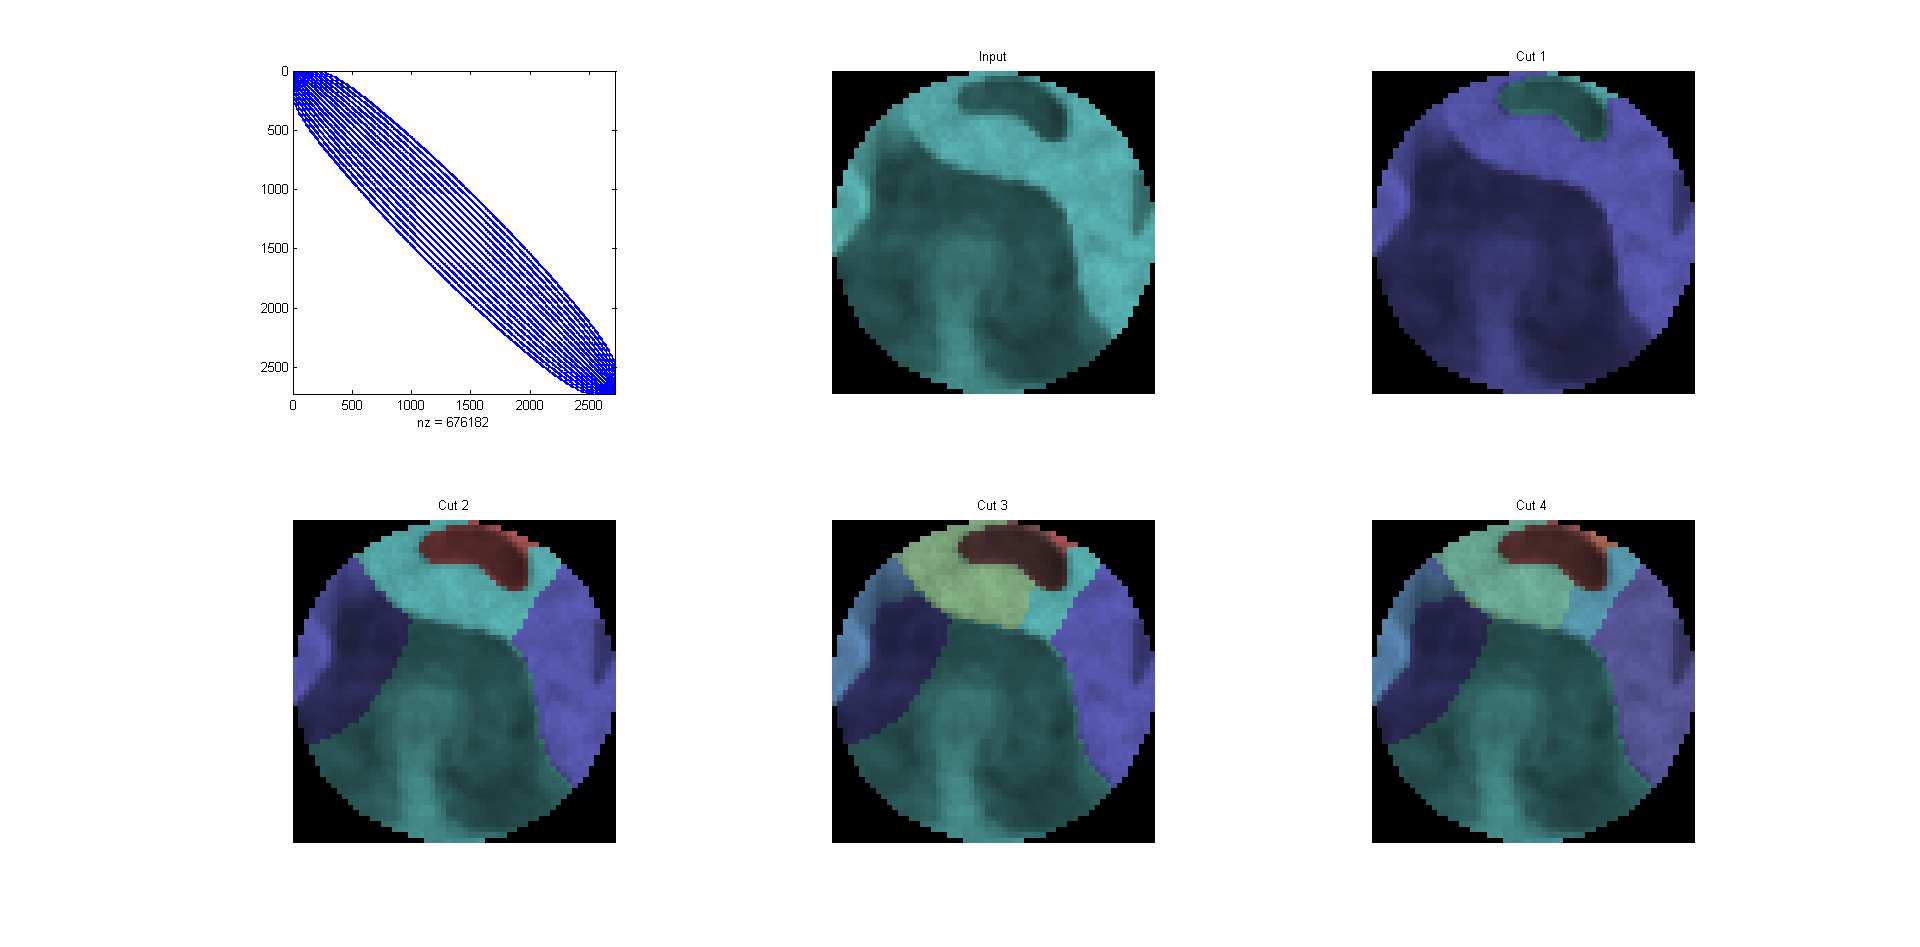
\includegraphics[width=0.6\linewidth,trim={5cm 2.5cm 5cm 1cm},clip]{imgs/eigen}
    \caption{\label{fig:eigen}
      System matrix $\mW$~and consecutive minimal normalized cuts on a simple example.
      Segments are colored randomly.
      For assignment to vertebra and filling cement, they will be broken into unconnected regions.}
  \end{figure}
  
    \begin{figure}[h]
      \centering
      \begin{subfigure}[t]{0.45\linewidth}
        \centering
        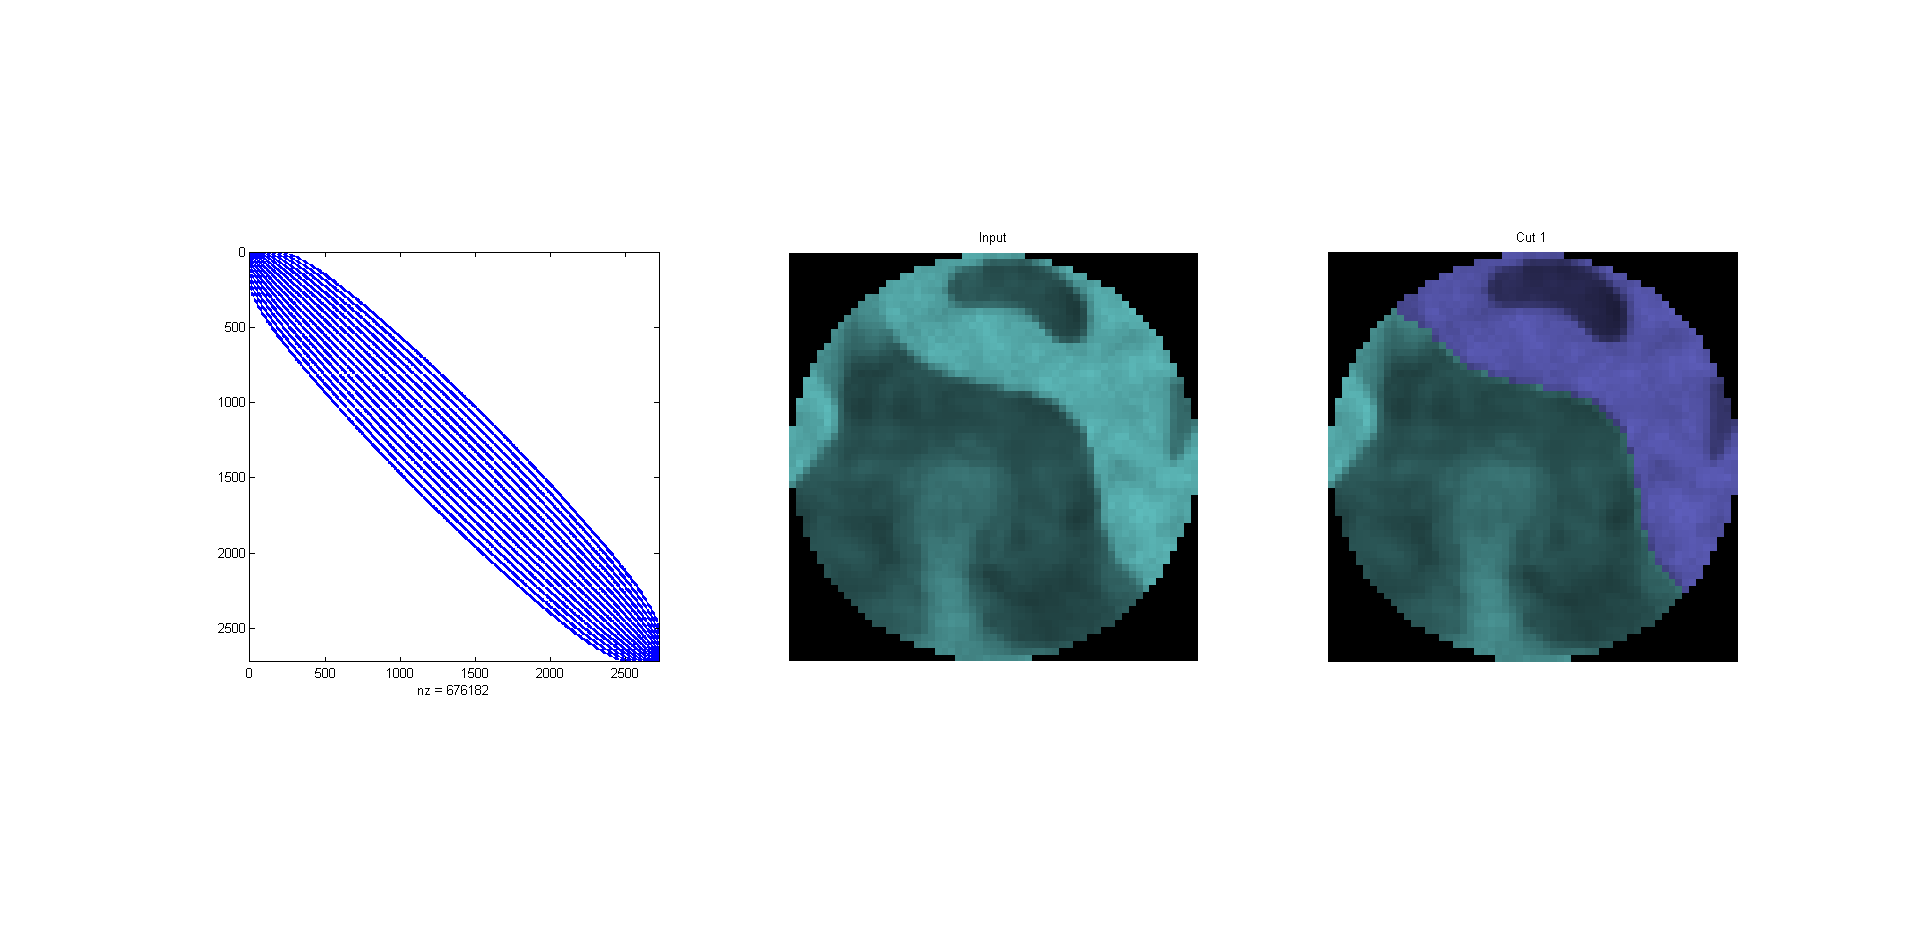
\includegraphics[width=\linewidth,trim={5cm 2.5cm 5cm 1cm},clip]{imgs/minvar1}
        \vspace{-1cm}
        \caption*{1st cut}
      \end{subfigure}
      \hfill
      \begin{subfigure}[t]{0.45\linewidth}
        \centering
        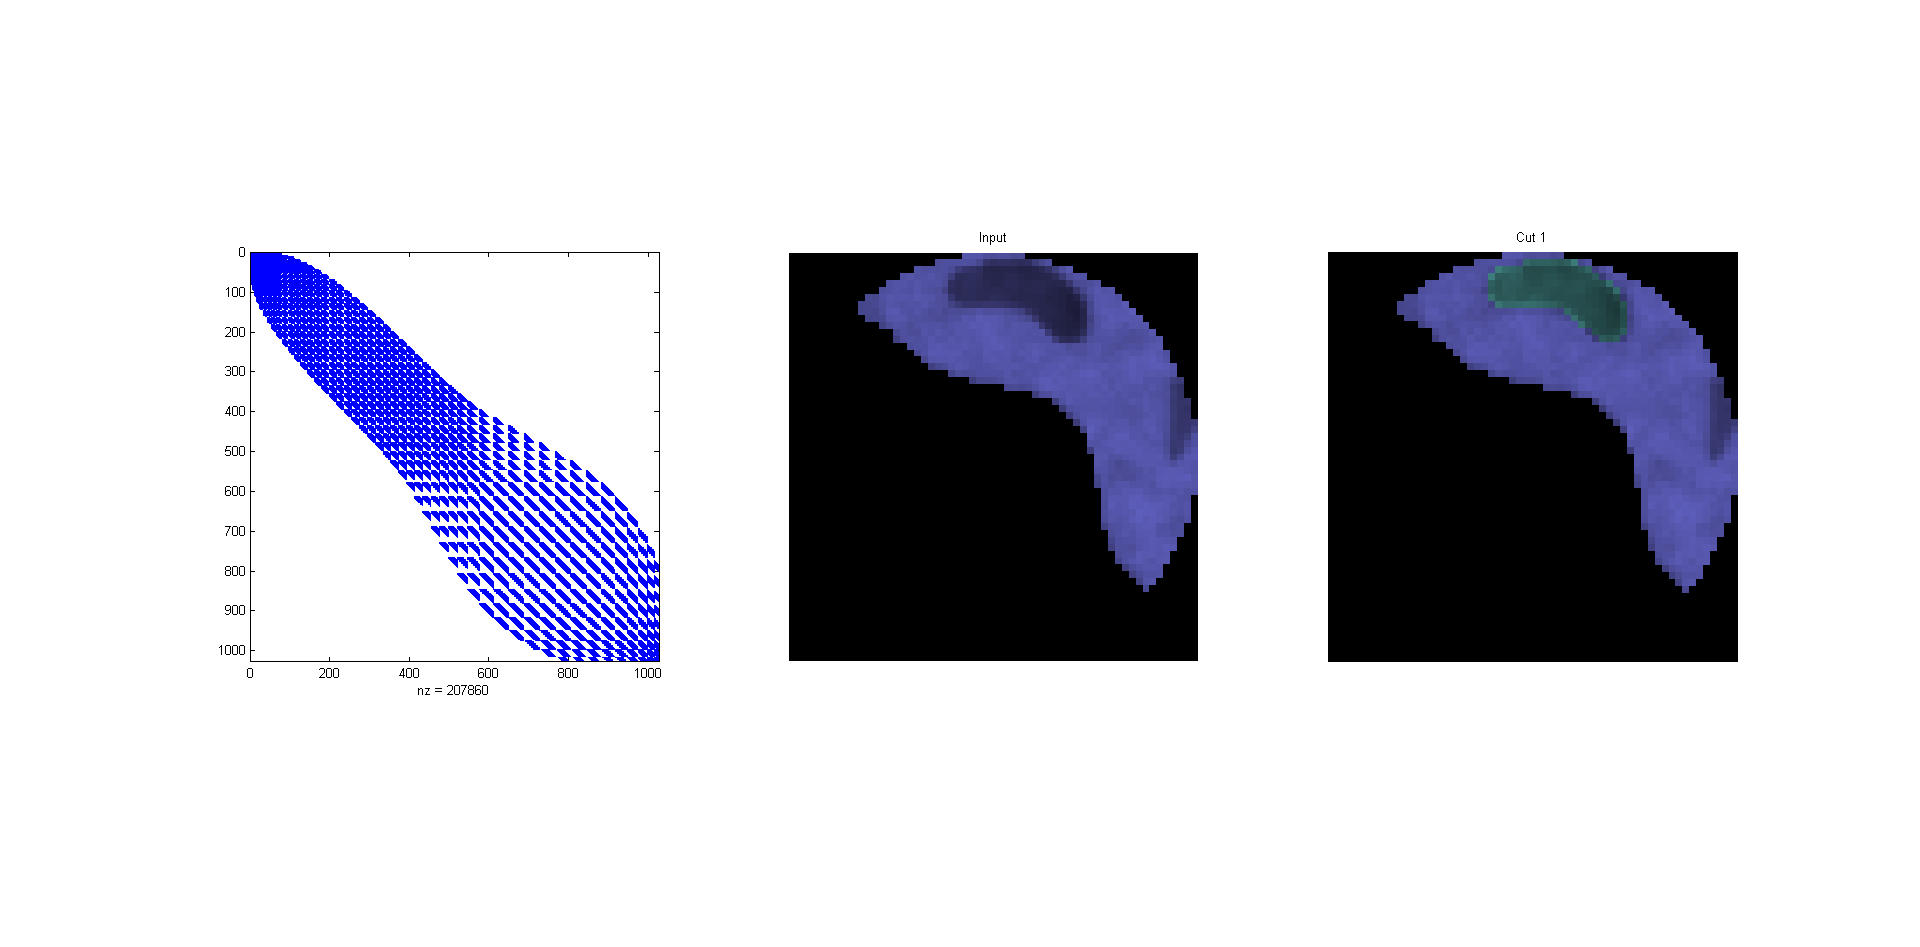
\includegraphics[width=\linewidth,trim={5cm 2.5cm 5cm 1cm},clip]{imgs/minvar2}
        \vspace{-1cm}
        \caption*{2nd cut}
      \end{subfigure}
      \vspace{-1cm}
      \begin{subfigure}[t]{0.45\linewidth}
        \centering
        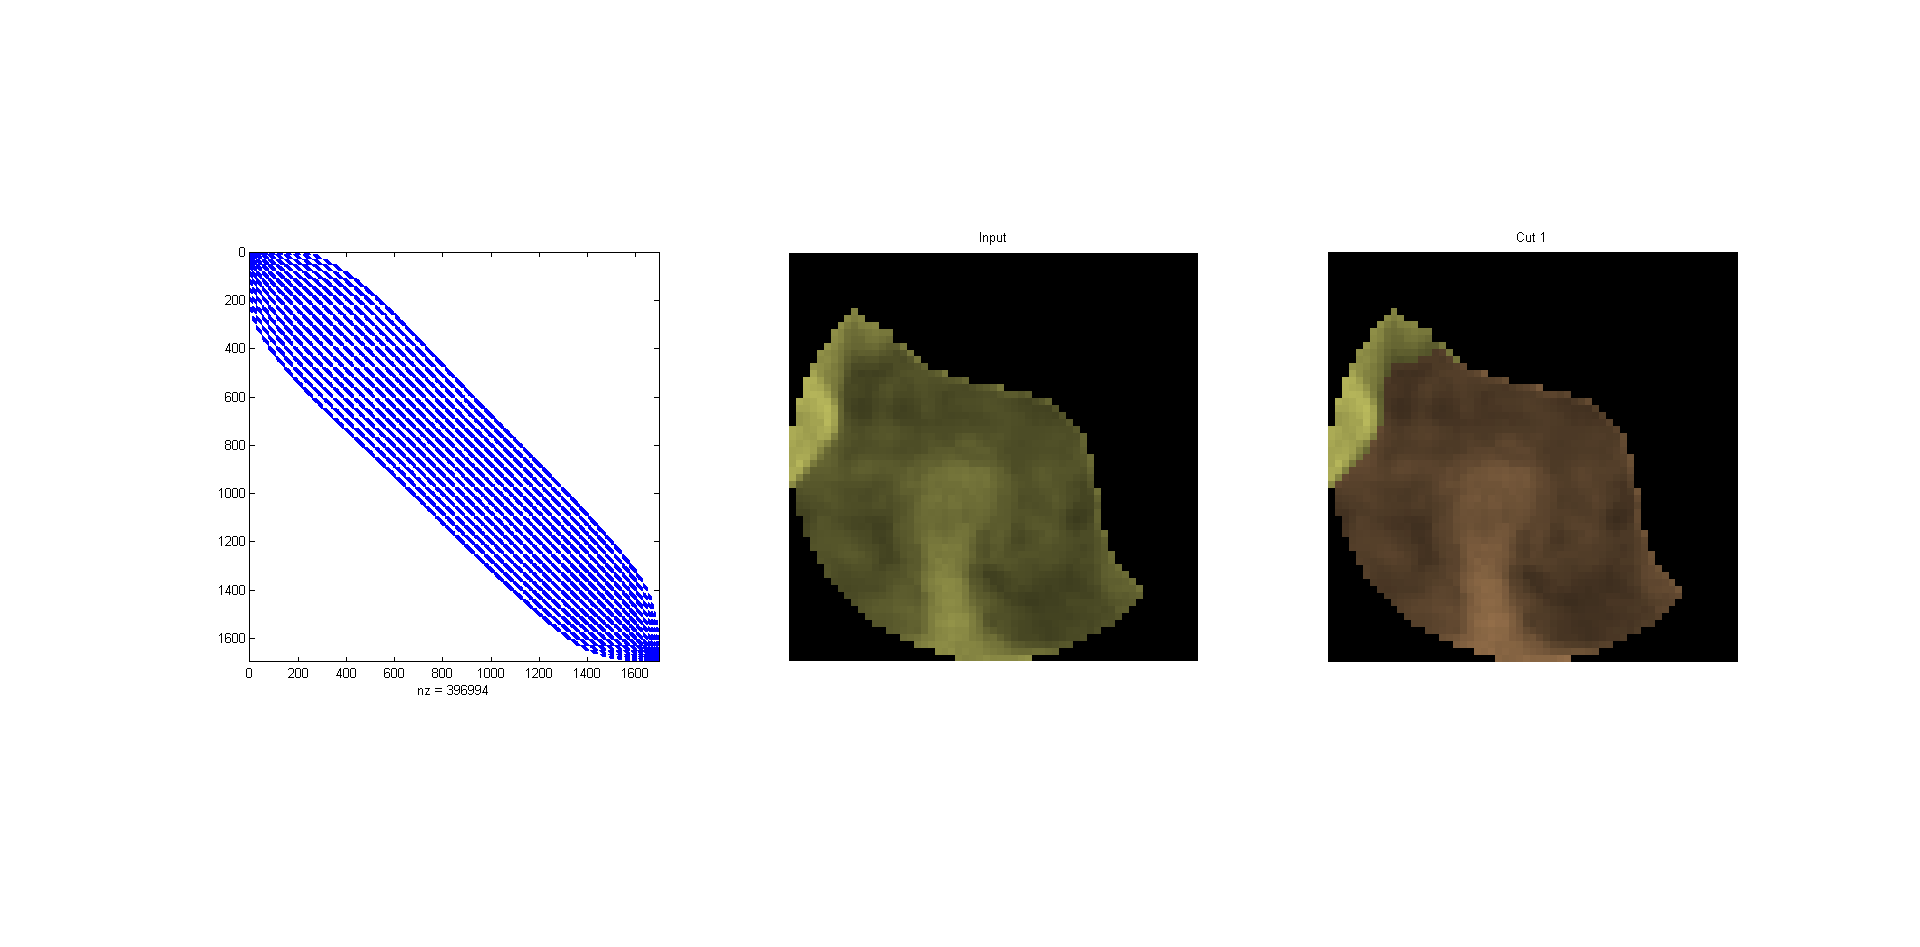
\includegraphics[width=\linewidth,trim={5cm 2.5cm 5cm 1cm},clip]{imgs/minvar3}
        \vspace{-1cm}
        \caption*{3rd cut}
      \end{subfigure}
      \hfill
      \begin{subfigure}[t]{0.45\linewidth}
        \centering
        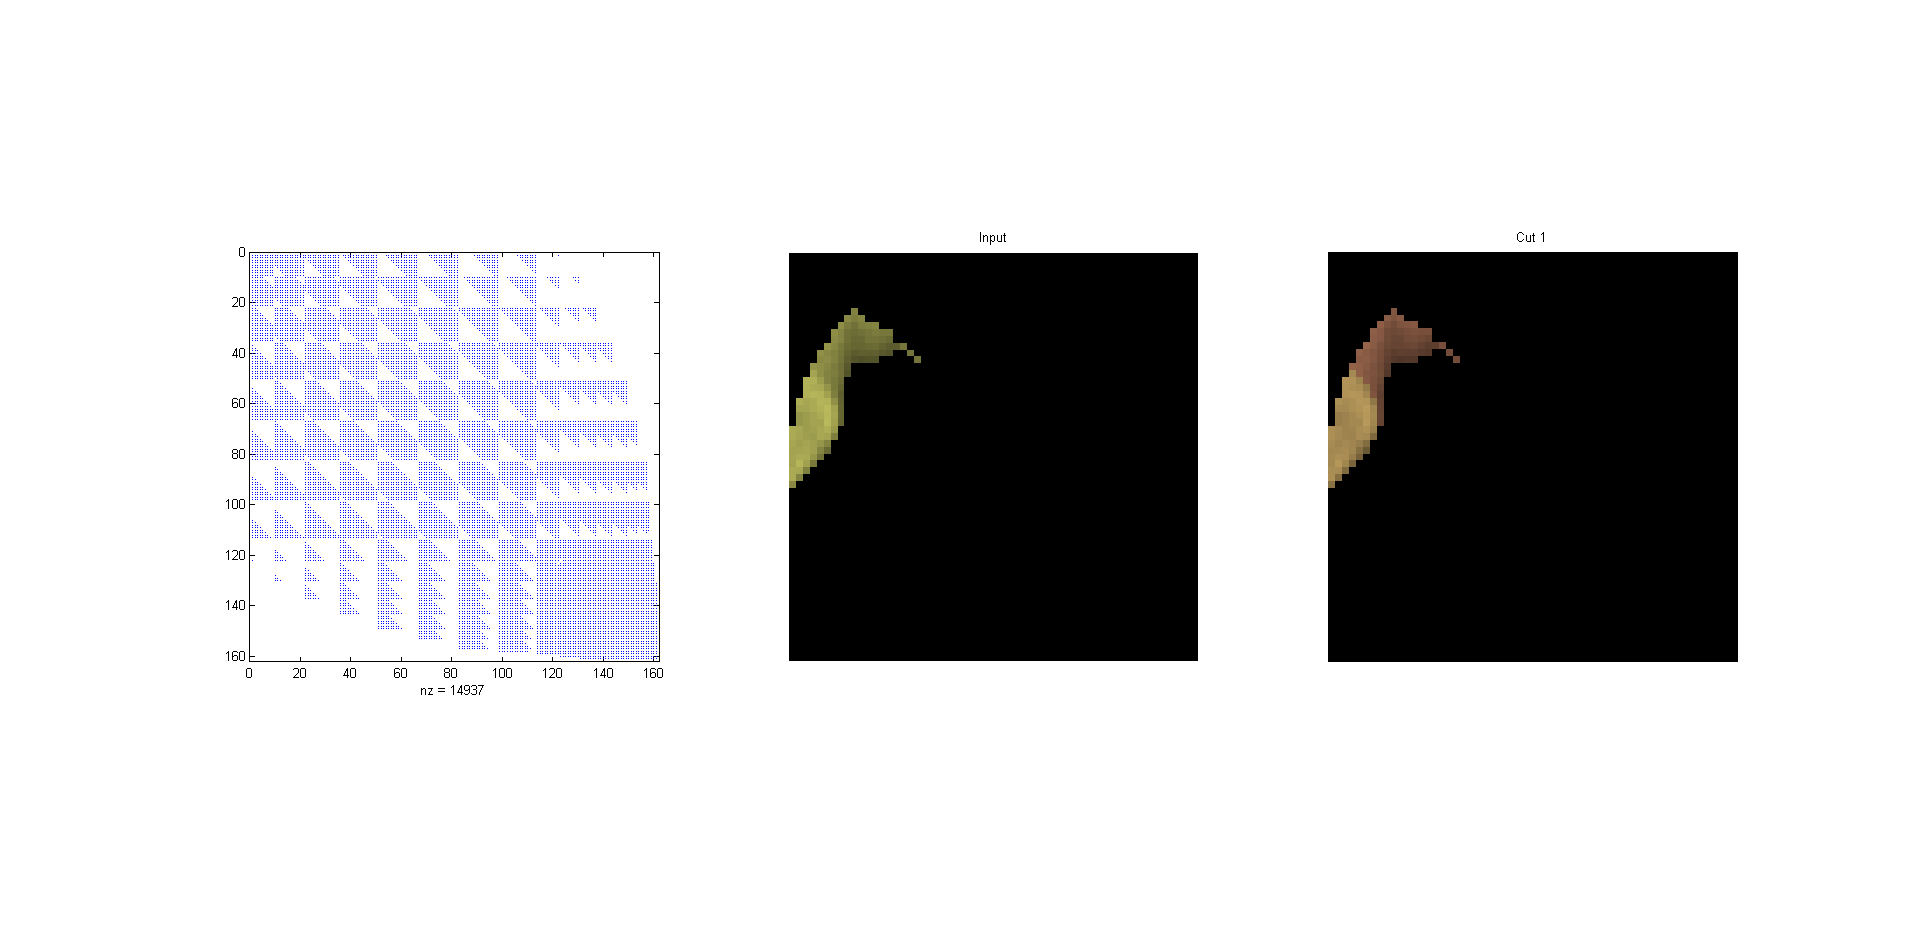
\includegraphics[width=\linewidth,trim={5cm 2.5cm 5cm 1cm},clip]{imgs/minvar4}
        \vspace{-1cm}
        \caption*{4th cut}
      \end{subfigure}
      \vspace{1cm}
      \caption{\label{fig:minvar}
        System matrix $\mW$, chosen segment for cutting and consecutive minimal normalized cut on a simple example.
        Segments are colored randomly.
        For assignment to vertebra and filling cement, they will be broken into unconnected regions.}
    \end{figure}
  
  The recursive variant is outperformed by both the equal area and minimal variance criterion.
  We further observed the cement regions to be rather small compared to the complete vertebra, and thus favor the fourth variance-based approach.
  
  The beauty lies in the applicability of the approach to different inputs, in our case 2D and 3D images.
  We were easily able to develop and debug on 2D images, as the extension to 3D could be achieved with a larger neighborhood and adjustments in the visualization.
  However, the additional dimension considerably adds to the computation speed and number of required cuts.
  
  
  
  \section{Results}
  {
    \begin{figure}[h]
      \centering
      \begin{subfigure}[t]{0.15\linewidth}
        \centering
        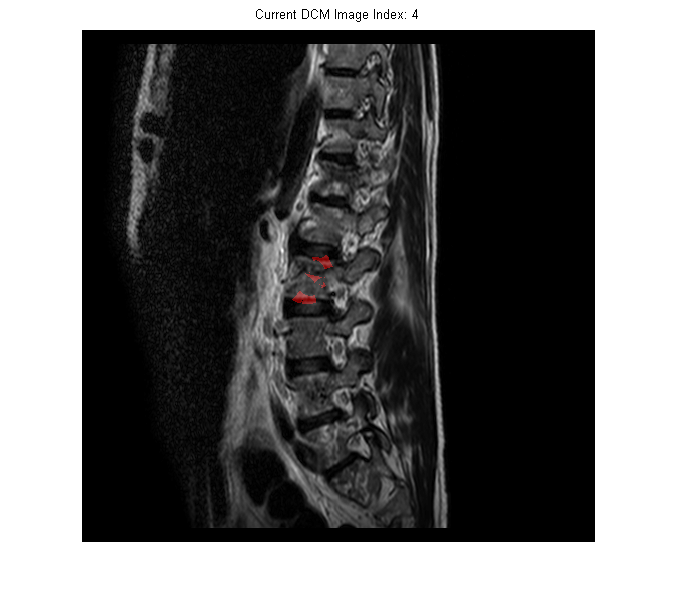
\includegraphics[width=\linewidth,trim={6cm 3cm 6cm 0},clip]{imgs/mask04}
      \end{subfigure}
      \hfill
      \begin{subfigure}[t]{0.15\linewidth}
        \centering
        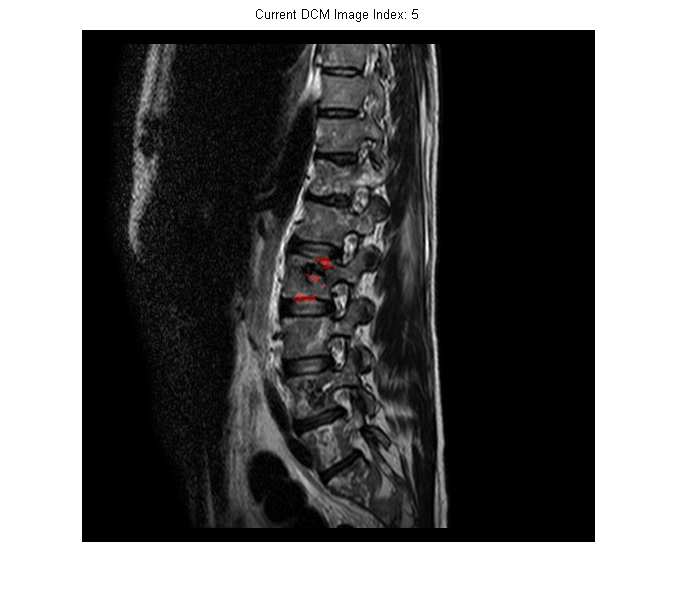
\includegraphics[width=\linewidth,trim={6cm 3cm 6cm 0},clip]{imgs/mask05}
      \end{subfigure}
      \hfill\begin{subfigure}[t]{0.15\linewidth}
        \centering
        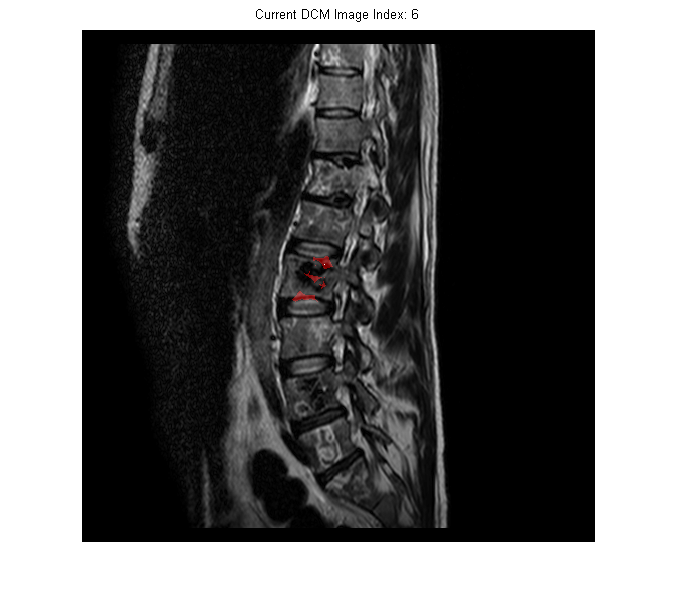
\includegraphics[width=\linewidth,trim={6cm 3cm 6cm 0},clip]{imgs/mask06}
      \end{subfigure}
      \hfill\begin{subfigure}[t]{0.15\linewidth}
        \centering
        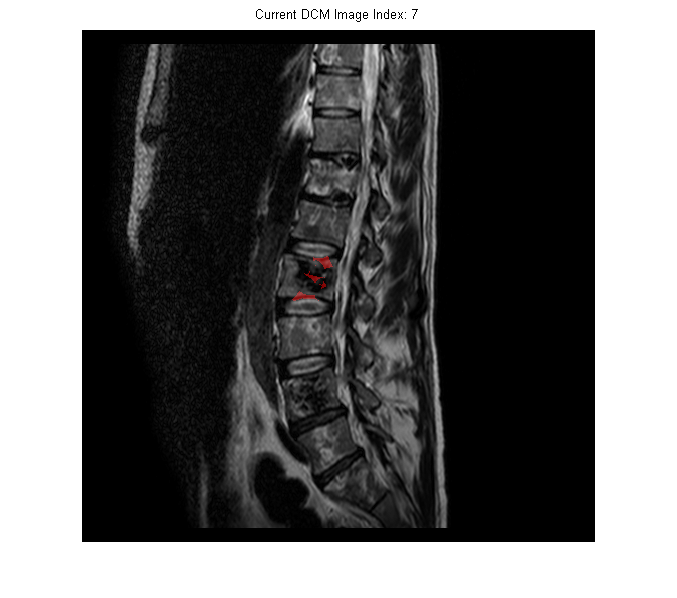
\includegraphics[width=\linewidth,trim={6cm 3cm 6cm 0},clip]{imgs/mask07}
      \end{subfigure}
      \hfill\begin{subfigure}[t]{0.15\linewidth}
        \centering
        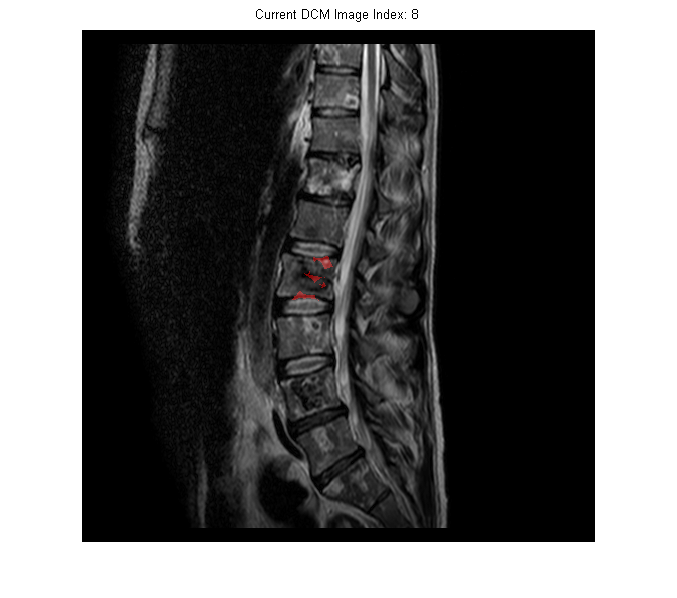
\includegraphics[width=\linewidth,trim={6cm 3cm 6cm 0},clip]{imgs/mask08}
      \end{subfigure}
      \hfill
      \begin{subfigure}[t]{0.15\linewidth}
        \centering
        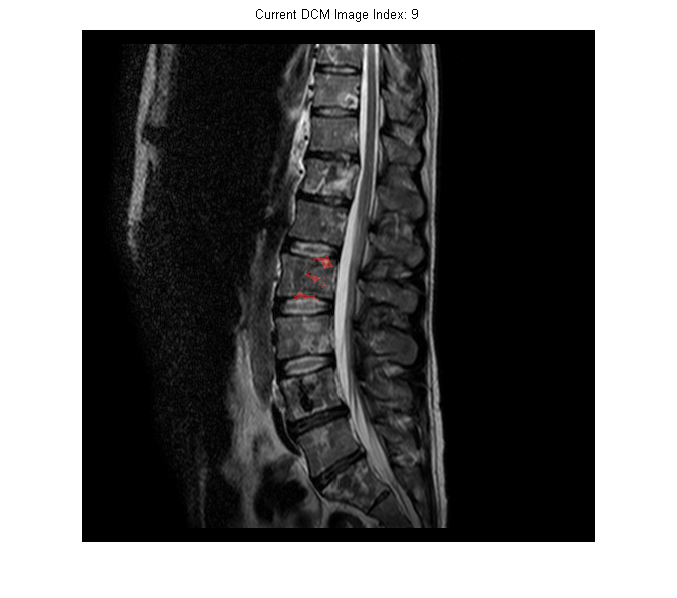
\includegraphics[width=\linewidth,trim={6cm 3cm 6cm 0},clip]{imgs/mask09}
      \end{subfigure}
      \vspace{.5cm}
      
      \begin{subfigure}[t]{0.15\linewidth}
        \centering
        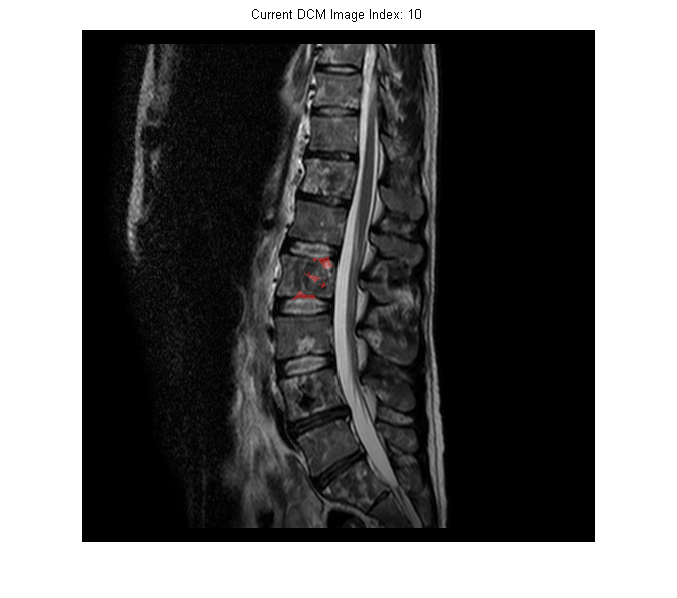
\includegraphics[width=\linewidth,trim={6cm 3cm 6cm 0},clip]{imgs/mask10}
      \end{subfigure}
      \hfill
      \begin{subfigure}[t]{0.15\linewidth}
        \centering
        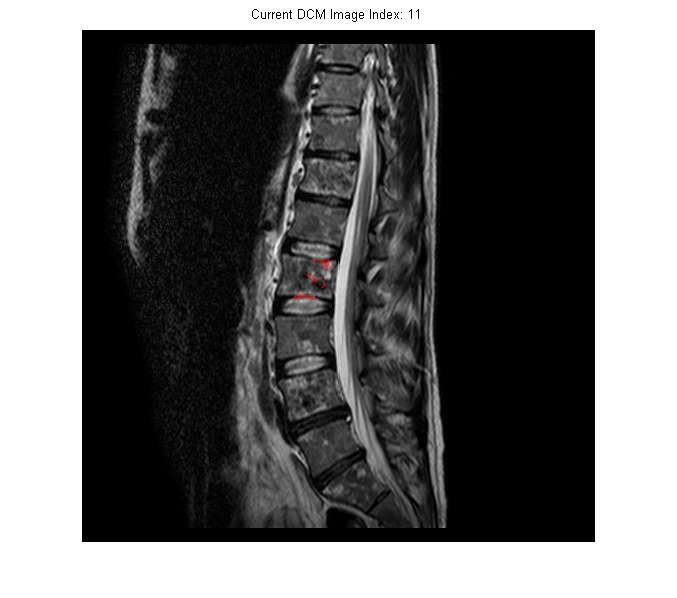
\includegraphics[width=\linewidth,trim={6cm 3cm 6cm 0},clip]{imgs/mask11}
      \end{subfigure}
      \hfill\begin{subfigure}[t]{0.15\linewidth}
        \centering
        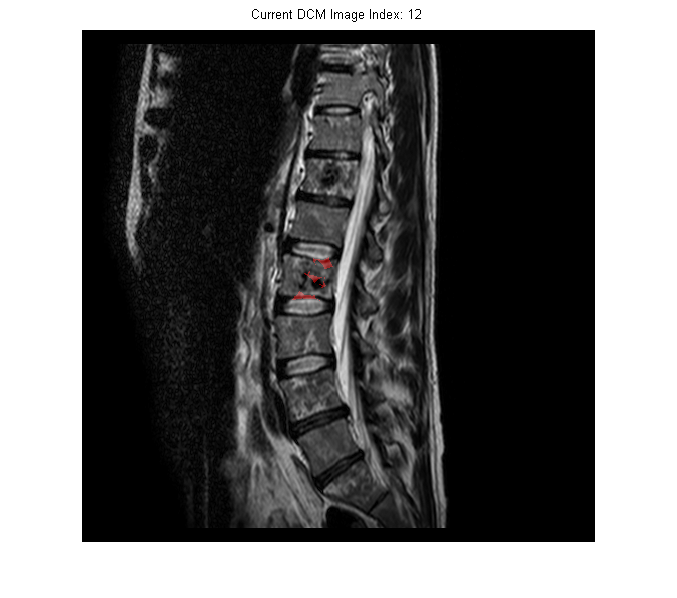
\includegraphics[width=\linewidth,trim={6cm 3cm 6cm 0},clip]{imgs/mask12}
      \end{subfigure}
      \hfill\begin{subfigure}[t]{0.15\linewidth}
        \centering
        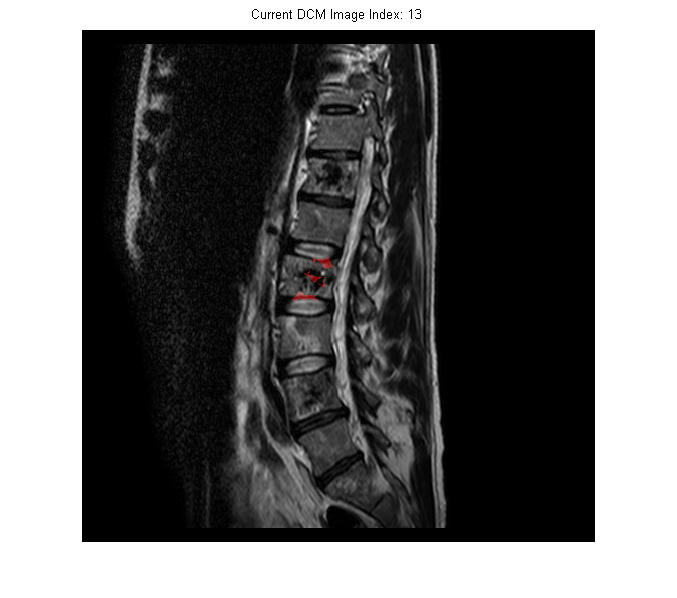
\includegraphics[width=\linewidth,trim={6cm 3cm 6cm 0},clip]{imgs/mask13}
      \end{subfigure}
      \hfill\begin{subfigure}[t]{0.15\linewidth}
        \centering
        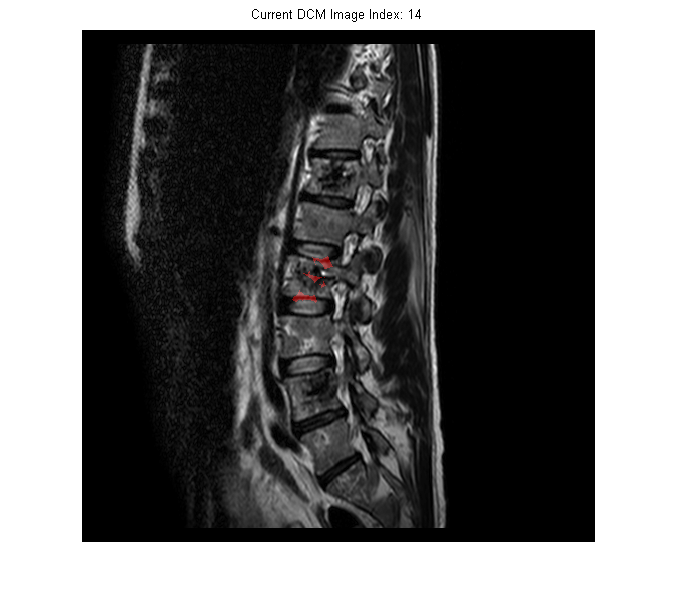
\includegraphics[width=\linewidth,trim={6cm 3cm 6cm 0},clip]{imgs/mask14}
      \end{subfigure}
      \hfill
      \begin{subfigure}[t]{0.15\linewidth}
        \centering
        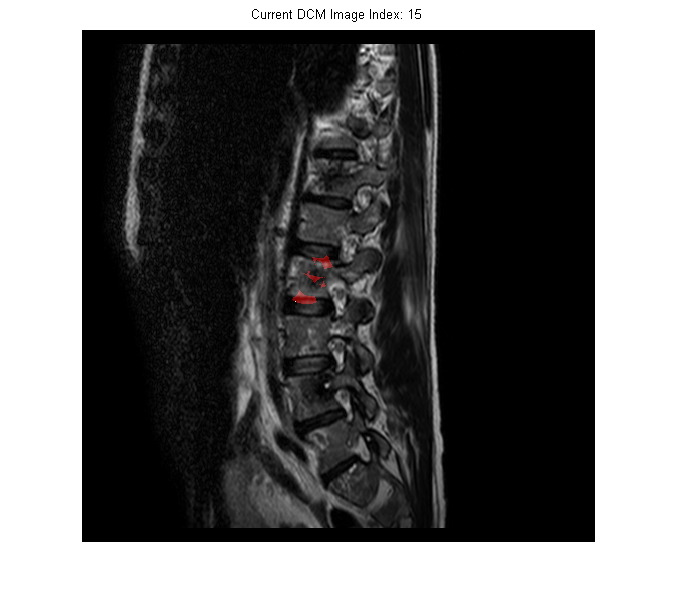
\includegraphics[width=\linewidth,trim={6cm 3cm 6cm 0},clip]{imgs/mask15}
      \end{subfigure}
      
      \caption{\label{fig:mask}
      Resulting segmentation of the central vertebra body in dataset $501/601$. Segmented cement is highlighted in red.\\
      Neighborhood up to $\pm~3 \times \pm~3 \times \pm~2$, $12$ cuts (up to $2^{12}~=~4096$ segments)}
    \end{figure}
  }
  
  In figure~\ref{fig:mask}, the segmentation results are shown over all slices containing the vertebra.
  We observed the mask to vary only slightly across the slices, which is probably due to the low connectivity and small neighborhood in this direction.
  The mask is thus not a good fit for the data.
  
  As our segmentation is obviously not suited for this task, we did not perform any additional comparison with the reference data given.
  
      \begin{figure}[h]
        \centering
        \begin{subfigure}[t]{0.48\linewidth}
          \centering
          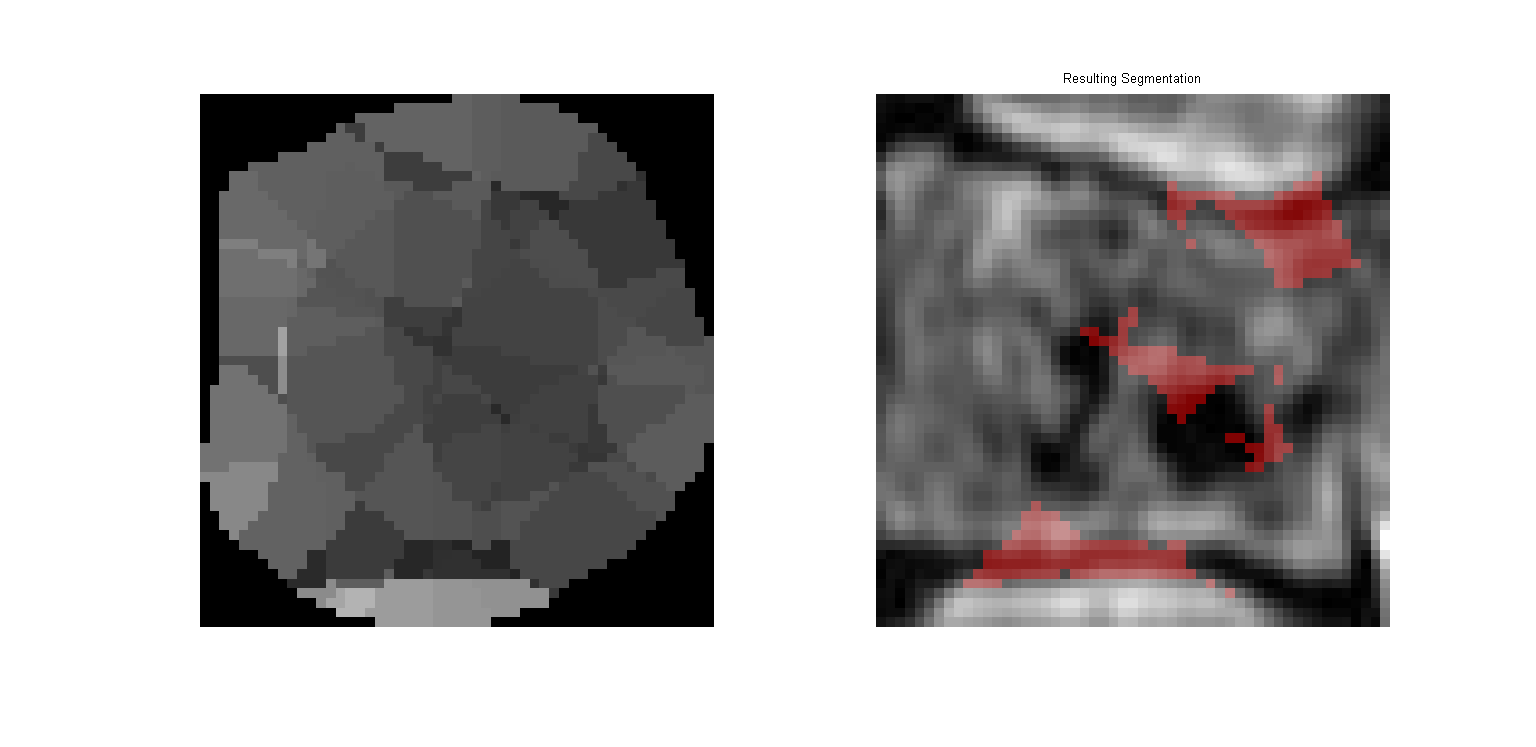
\includegraphics[width=\linewidth,trim={5cm 4cm 5cm 1cm},clip]{imgs/vars12}
          \caption{Slice of 3D segmentation\\
            Neighborhood up to $\pm~3 \times \pm~3 \times \pm~2$, $12$ cuts (up to $2^{12}~=~4096$ segments with multiple unconnected regions)
          }
        \end{subfigure}
        \hfill
        \begin{subfigure}[t]{0.48\linewidth}
          \centering
          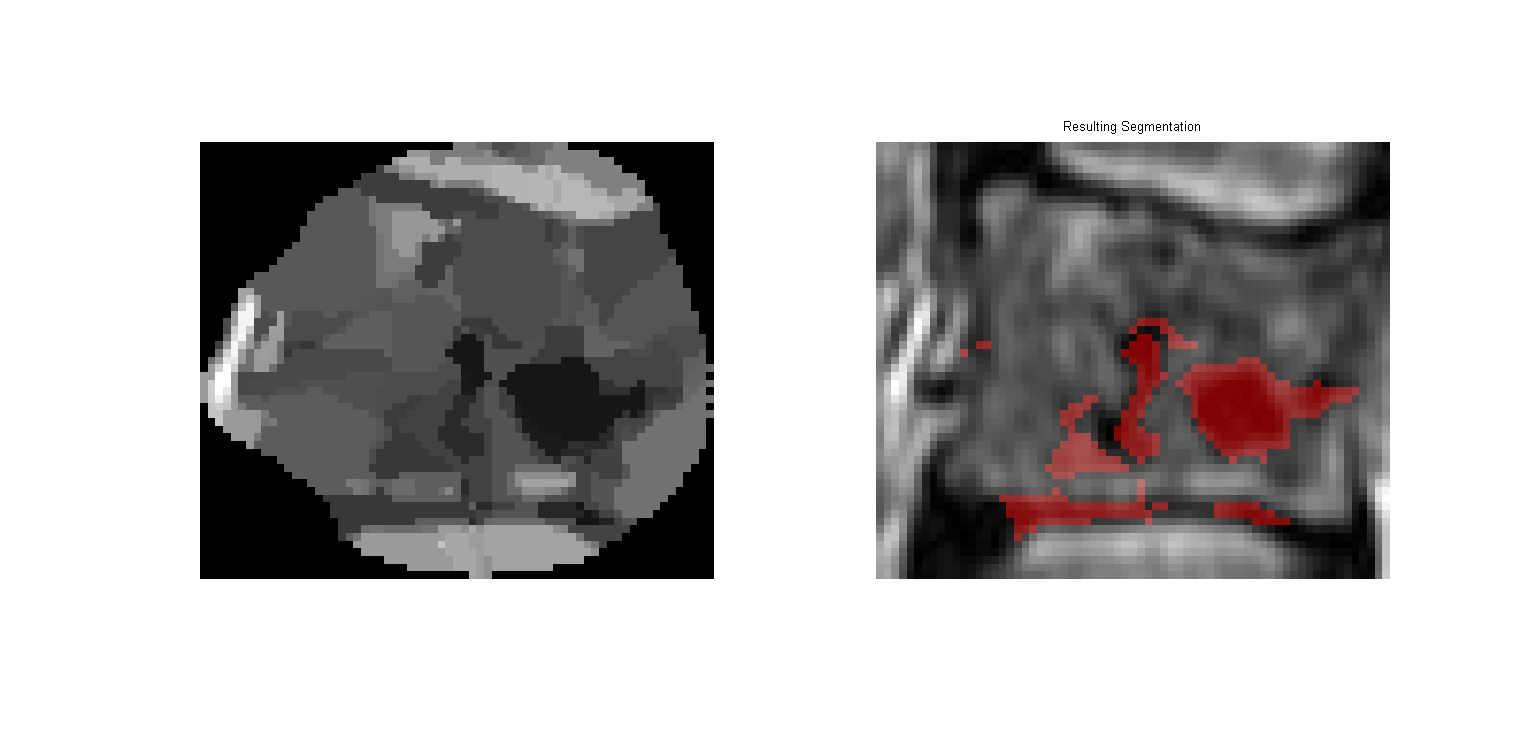
\includegraphics[width=\linewidth,trim={5cm 2.6cm 5cm 2.4cm},clip]{imgs/vars12-2D}
          \caption{Results from 2D segmentation on slice\\
            Neighborhood up to $\pm~8 \times \pm~8$, $4$ cuts a time, $5$ iteration, minimizing variance (up to $24$ segments with multiple unconnected regions)
          }
        \end{subfigure}
        \caption{\label{fig:2D3D}
          Segments colored by mean value and masked data, all in slice $12$.
          Though way fewer segments were created in (b), the fit is better.}
      \end{figure}
      
  For comparison, in figure~\ref{fig:2D3D} 
  
%  \pagebreak
  \section{Evaluation}
  
  
  \begin{thebibliography}{9}
    
    \bibitem{[ChanVese01]}
    T. F. Chan and L. A. Vese,
    \emph{"Active contours without edges", IEEE Transactions on Image Processing},
    vol. 10, Issue 2, pp. 266-277, 2001.
    
    
    \bibitem{[ShiMalik00]}
    J.  Shi  and  J.  Malik,
    \emph{"Normalized Cuts and Image Segmentation", IEEE Transactions on Pattern Analysis and Machine Intelligence},
    vol. 22, pp.888-904,
    2000.
    
    \bibitem{[MumfordShah89]}
    D. Mumford and J. Shah,
    \emph{Optimal approximation by piecewise smooth functions and associated
      variational problems," Communications on Pure and Applied Mathematics},
    vol. 42, pp. 577-685,,
    1989.
    
  \end{thebibliography}
  
\end{document}